\section{Desenvolvimento}

Já desde o início de janeiro, a proposta inicial do \calopsita{} foi montada. Durante o mês de janeiro, as tecnologias que poderiam ser interessantes no desenvolvimento do projeto foram estudadas e conseguiu-se o apoio do professor Alfredo Goldman, que aceitou orientar a equipe, da Caelum, que cedeu horas de trabalho para os desenvolvedores e dos mestrandos Mariana Bravo e Hugo Corbucci, os clientes eleitos.

Também desde então há o grupo de discussões~\footnote{http://groups.google.com/group/calopsita-development} e um repositório no GitHub para o projeto~\footnote{http://github.com/caelum/calopsita}. Esse repositório foi movido durante o desenvolvimento, mas seu histórico completo se manteve. Na figura \ref{figura:github}, vê-se um gráfico de número de linhas enviadas ao repositório no decorrer do ano. Ele ilustra a distribuição da geração de código ao longo do ano.

\begin{figure}[H]
  \centering
  \fbox{
    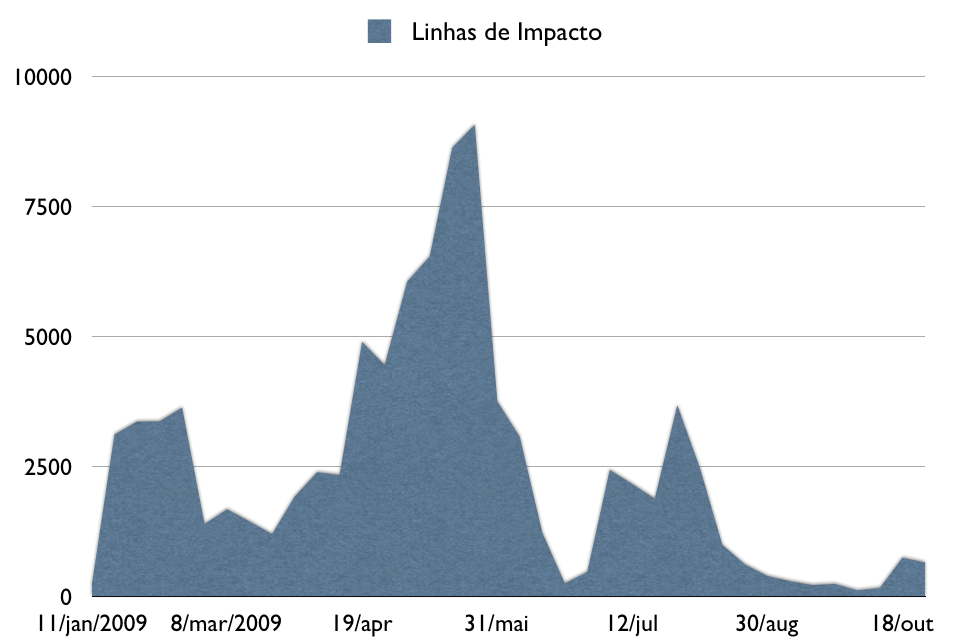
\includegraphics[width=110mm]{images/impacto.png}
  }
  \caption{Linhas de impacto - GitHub}\label{figura:github}
\end{figure}

Esses dados foram coletados do gráfico de impacto do GitHub e as divisões de linhas por desenvolvedor foram removidas porque, como a equipe adota programação pareada na maioria do tempo, as divisões não necessariamente representam a participação única de cada desenvolvedor no projeto.

Nota-se, dessa imagem, um pico de linhas de código enviadas ao repositório no mês de maio, mês seguinte a quando passou-se a gerenciar o próprio \calopsita{} usando a parte que já estava pronta do projeto. Contudo, houve trabalho de janeiro até o momento atual, com uma considerável queda em setembro para que focássemos nessa monografia.

Esse fenômeno é bastante natural: quando começa-se a usar um sistema novo, encontra-se diversos problemas e pontos de melhoria. A pressa para resolver os problemas mais impeditivos demandou um esforço maior da equipe.

\subsection{Gerenciamento do projeto}

Por tratar-se de um projeto de médio porte, seria indicado optar por alguma metodologia de gerenciamento de \software{}. Métodos tradicionais nem sequer foram considerados. Há algumas razões para isso.

Primeiramente porque, buscando informações históricas sobre o modelo \textit{Waterfall}, descobriu-se que mesmo o artigo~\cite{waterfall} que primeiro descreveu o modelo avisava que sua implementação é quase utópica e propensa a falhas.

\begin{quote}
\textit{``I believe in this concept, but the implementation described above is risky and invites failure.'}'
\end{quote}

Mais do que isso, o autor, já em 1970, sugeria que o desenvolvimento iterativo é mais apropriado para o desenvolvimento de projetos de \software{}. Isso apenas aumenta a consternação com relação ao que é ensinado em universidades ao redor do mundo e se vê no mercado de trabalho ainda hoje -- diversas empresas que clamam usar RUP~\cite{rup} ignoram sua parte mais importante, o desenvolvimento iterativo.

Em segundo lugar, métodos tradicionais prezam pelo conhecido \textit{``Big Design Up Front'}', isto é, em planejar toda a arquitetura de um sistema antes de começar a produzí-lo e manter esse \textit{design} até o produto final surgir. Essa ideia pressupõe que, de início, se saiba tudo o que será necessário do sistema e que essas necessidades não mudem. A experiência mostra que, na produção de \software{}, o padrão é não conhecer de antemão o que se precisa e as necessidades mudarem com o tempo~\cite{change}.

De fato, verificou-se a verdade nessa afirmação quando, no início do projeto, os clientes queriam um papel Administrador do Sistema no \calopsita{} que restringiria partes do sistema que podem ser editados por cada tipo de usuário. Essa funcionalidade, assim como diversas outras, acabou não sendo implementada por se mostrar desnecessária.

Finalmente, tanto os desenvolvedores quanto os clientes do \calopsita{} valorizam o \textit{feedback} rápido e atribuem a isso muitos projetos bem-sucedidos. Os clientes têm seus trabalhos de mestrado relacionados com métodos ágeis e anos de experiência nessas metodologias. Os desenvolvedores trabalham diariamente com Scrum~\cite{scrum} e XP~\cite{xp} e possuem certificações pela Scrum Alliance~\footnote{http://www.scrumalliance.org/}. 

A equipe, como um todo, acredita que as metodologias ágeis são uma resposta ao modo engessado com que métodos tradicionais tratam a produção de \software{} e que, aplicando os valores descritos no Manifesto Ágil~\cite{manifesto}, obtemos produtos de qualidade, que atendem às necessidades reais dos clientes e dão satisfação aos desenvolvedores.  

\subsection{Abordagem Ágil}

Embora Scrum não tenha sido usado para desenvolver o \calopsita{}, utilizamos alguns métodos e ferramentas típicos desse
\textit{framework} e de XP que melhor funcionavam para o time. O uso de metodologias e \textit{frameworks} são excelentes para
times e pessoas em migração das formas tradicionais, mas seu uso não se mostrou necessário no time do \calopsita{}. Todos,
clientes e desenvolvedores, têm grande experiência com métodos ágeis e, dessa forma, optou-se por simplesmente seguir os
preceitos ágeis e adaptar os métodos que ajudassem mais a cada etapa. 

\subsubsection*{Kanban~\cite{kanban}}

Como, durante a maior parte do desenvolvimento, os programadores trabalhavam no mesmo espaço físico, pôde-se adotar um quadro branco com \textit{kanban}, uma forma de organização de tarefas bastante difundida na área de Administração que foi portada para \software{} mais recentemente. A figura \ref{figura:kanban} mostra o quadro branco do Calopsita, com o \textit{kanban} à esquerda, visão, anotações e as \textit{personas} à direita -- essas últimas, serão explicadas mais adiante nessa seção.

\begin{figure}[H]
  \centering
  \fbox{
    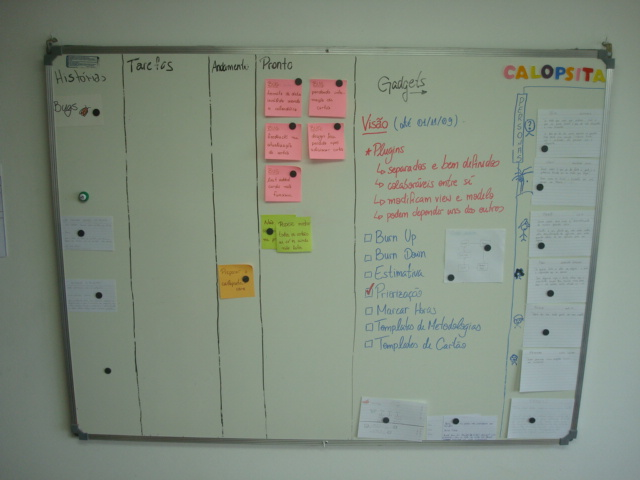
\includegraphics[width=110mm]{images/calopsita-kanban.png}
  }
  \caption{Kanban do \calopsita{}}\label{figura:kanban}
\end{figure}

O quadro branco é uma forma bastante eficiente de comunicação -- basta olhar para ele para entender, de imediato, o que há para ser feito, o que já está pronto e quais tarefas estão em andamento. Além disso, nosso quadro conta com a \textbf{Visão do Projeto}, isto é, a meta maior para o projeto, onde queremos chegar.

\subsubsection*{Integração Contínua}

Para manter o código funcional a cada mudança, utilizou-se, desde o começo do projeto, um servidor de integração contínua~\cite{ci}, o CruiseControl.rb~\footnote{http://cruisecontrolrb.thoughtworks.com/}. Esse servidor é capaz de consultar o repositório de código de tempos em tempos verificando por mudanças no código. Uma vez detectada alguma alteração, ele baixa o novo código, compila e roda seus testes de forma automática. Se durante esse processo qualquer um dos testes falhar, um email é disparado para toda a equipe, garantido que o bug introduzido seja corrigido o mais rapidamente possível. Por outro lado, se todos os testes forem executados com sucesso, um \textit{deploy} é feito de forma automática em um servidor de homologação. Isso permite que todos os envolvidos consigam acompanhar e testar, em tempo real, tudo que está sendo implementado. A figura \ref{figura:cruisecontrol} mostra resultados do processo no final de outubro de 2009.

\begin{figure}[H]
  \label{figura:cruisecontrol}
  \centering
  \fbox{
    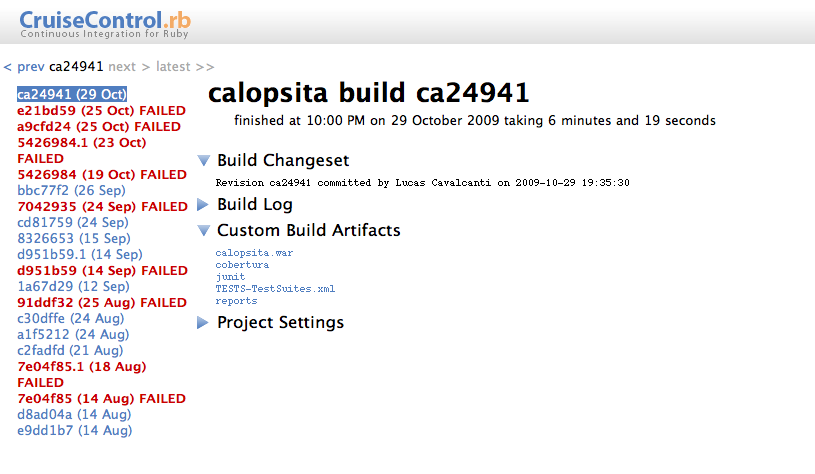
\includegraphics[width=110mm]{images/cruisecontrol-calopsita.png}
  }
  \caption{Cruisecontrol.rb do \calopsita{}}
\end{figure}

\subsubsection*{Pareamento e refatoração}

A qualidade do código, tanto em aspectos de legibilidade quanto em arquitetura, é assegurada por discussões técnicas na lista do projeto, por discussões com profissionais da Caelum e pelo uso extensivo de programação em pares. As vantagens da programação em pares~\cite{pair}, contudo, vão além da manutenção da qualidade de código -- atribuímos a essa prática o nivelamento do conhecimento não apenas sobre o código do Calopsita, mas também sobre os conceitos aplicados em diversas partes do sistema.

Outro fator que colaborou bastante na qualidade do código é a cultura de refatorações que a equipe adota. A regra é que, sempre que se encontra código que poderia ser melhor, melhora-se ele. Isso faz com que o código se mantenha sempre atual e o melhor possível na visão da equipe de desenvolvimento.

\subsubsection*{Interação com clientes}

Para manter o foco do projeto no que era mais valioso para o cliente a cada momento, a interação com esses foi fundamental para o bom andamento do projeto. Houve reuniões semanais ou quinzenais durante todo o ano, onde os clientes testavam o \calopsita{} ambiente de homologação, aprovavam tarefas,  repriorizavam os cartões de funcionalidades e definiam uma meta para a iteração seguinte. 

Com a estabilização do \calopsita{}, diversos projetos da Caelum também começaram a usar o sistema para gerência dos ítens por fazer e iterações. Assim, passamos a ter mais clientes e, portanto, mais pedidos de funcionalidades e correções. Nesse momento, usar o próprio \calopsita{} para auxiliar em seu desenvolvimento se mostrou bastante conveniente: os clientes colocavam seus pedidos no sistema e priorizavam seus cartões.

\subsubsection*{Personas}

Trabalhando com diversos clientes traz um aumento considerável na complexidade de comunicação entre as partes envolvidas no projeto. Tanto a comunicação entre clientes diferentes quanto com a equipe de desenvolvimento foi facilitada com o uso de \textit{Personas}. Os pedidos eram feitos em nome de um personagem cujos valores eram conhecidos pela equipe e pelos clientes. 

Por exemplo, a \textit{persona} \textit{Fabs} representa um usuário do sistema que é um tanto distraído e quer que o sistema não tenha ambiguidades que possam confundí-lo. Com essa descrição, todos sabem que essa persona representa a preocupação com usabilidade e interação homem-computador. Um cartão desse personagem, tirado do \textit{backlog} do \calopsita{}, pode ser visto a seguir, no cartão \ref{tabela:fabs}.

\begin{figure}[H]
  \label{tabela:fabs}
  \begin{tabular}{|p{10cm}|}
    \hline
    Para não me confundir sobre qual cartão eu peguei \\
    Como Fabs \\
    Quero que os cartões na priorização e na iteração mantenham a mesma forma quando são arrastados. \\
    \hline
  \end{tabular}
\end{figure}

A lista e descrições das \textit{personas} usadas na construção do \calopsita{} podem ser encontradas no apêndice~\ref{sec:personas}.
